% MedVision manuscript -- Results section

\section{Results}\label{sec:results}

\subsection{Analysis set and output completeness}\label{sec:results-completeness}
The fixed-merge archive contained 40 model--seed records (five conditions and
eight seeds), each evaluated on the same 455 held-out studies. Single retained
outputs were available for image-only, text-only, and Gray-Square controls.
GACR-B was post hoc and exploratory. Duplicate keys were resolved by the
first-seen archive value; because a deterministic source-priority rule and hash
manifest were not preserved, results remain tied to this snapshot. ECE and
Brier score were recomputed from probability arrays in the companion pickle
because the JSON summary omitted them. All confirmatory comparisons were paired
at seed level; repeated test studies were not concatenated across seeds.

\subsection{Predictive performance and calibration}\label{sec:results-primary}
Baseline CADQ achieved Macro-F1 $0.9397\pm0.0061$, accuracy
$0.9607\pm0.0032$, and Macro-AUROC $0.9974\pm0.0004$ (Table~\ref{tab:primary-performance}).
LMH had the highest Macro-F1 ($0.9435\pm0.0093$) but lower, more variable
AUROC ($0.9849\pm0.0113$). Noise-Consistency had the lowest confirmatory
Macro-F1 ($0.9346\pm0.0075$); Adaptive-CADQ was close to baseline. Exploratory
GACR-B reached $0.9417\pm0.0059$.

\begin{table}[pos=htbp]
\centering
\caption{Primary test-set performance across eight seeds (mean $\pm$ standard
deviation [SD]).
GACR-B was exploratory and post hoc.}
\label{tab:primary-performance}
\small
\begin{tabular}{lccc}
\toprule
Condition & Macro-F1 & Accuracy & Macro-AUROC\\
\midrule
Baseline CADQ       & 0.9397 $\pm$ 0.0061 & 0.9607 $\pm$ 0.0032 & 0.9974 $\pm$ 0.0004\\
LMH                 & 0.9435 $\pm$ 0.0093 & 0.9596 $\pm$ 0.0070 & 0.9849 $\pm$ 0.0113\\
Noise-Consistency   & 0.9346 $\pm$ 0.0075 & 0.9560 $\pm$ 0.0039 & 0.9960 $\pm$ 0.0013\\
GACR-B (exploratory)& 0.9417 $\pm$ 0.0059 & 0.9610 $\pm$ 0.0042 & 0.9972 $\pm$ 0.0005\\
Adaptive-CADQ      & 0.9388 $\pm$ 0.0072 & 0.9610 $\pm$ 0.0044 & 0.9972 $\pm$ 0.0008\\
\bottomrule
\end{tabular}
\end{table}

Baseline per-class F1 was 0.9755 for Normal, 0.9624 for Pneumonia, and 0.8810
for Pneumothorax (Table~\ref{tab:calibration-class}). LMH improved Pneumothorax
F1 to 0.9003 but reduced Pneumonia F1 to 0.9575. Noise-Consistency had the
widest Pneumothorax variation; Adaptive-CADQ had the most stable Pneumonia F1.

\begin{table}[pos=htbp]
\centering
\caption{Calibration and per-class F1 across eight seeds (mean $\pm$ SD).}
\label{tab:calibration-class}
\scriptsize
\begin{tabular}{lccccc}
\toprule
Condition & ECE & Brier & Normal F1 & Pneumonia F1 & Pneumothorax F1\\
\midrule
Baseline CADQ        & 0.0237 $\pm$ 0.0048 & 0.0522 $\pm$ 0.0040 & 0.9755 $\pm$ 0.0032 & 0.9624 $\pm$ 0.0055 & 0.8810 $\pm$ 0.0174\\
LMH                  & 0.0621 $\pm$ 0.0160 & 0.0685 $\pm$ 0.0213 & 0.9726 $\pm$ 0.0066 & 0.9575 $\pm$ 0.0077 & 0.9003 $\pm$ 0.0191\\
Noise-Consistency    & 0.0347 $\pm$ 0.0137 & 0.0655 $\pm$ 0.0130 & 0.9754 $\pm$ 0.0044 & 0.9530 $\pm$ 0.0058 & 0.8753 $\pm$ 0.0237\\
GACR-B (exploratory) & 0.0245 $\pm$ 0.0023 & 0.0540 $\pm$ 0.0038 & 0.9741 $\pm$ 0.0043 & 0.9630 $\pm$ 0.0066 & 0.8880 $\pm$ 0.0167\\
Adaptive-CADQ       & 0.0241 $\pm$ 0.0070 & 0.0527 $\pm$ 0.0028 & 0.9776 $\pm$ 0.0054 & 0.9616 $\pm$ 0.0029 & 0.8772 $\pm$ 0.0175\\
\bottomrule
\end{tabular}
\end{table}

\begin{figure}[pos=htbp]
\centering
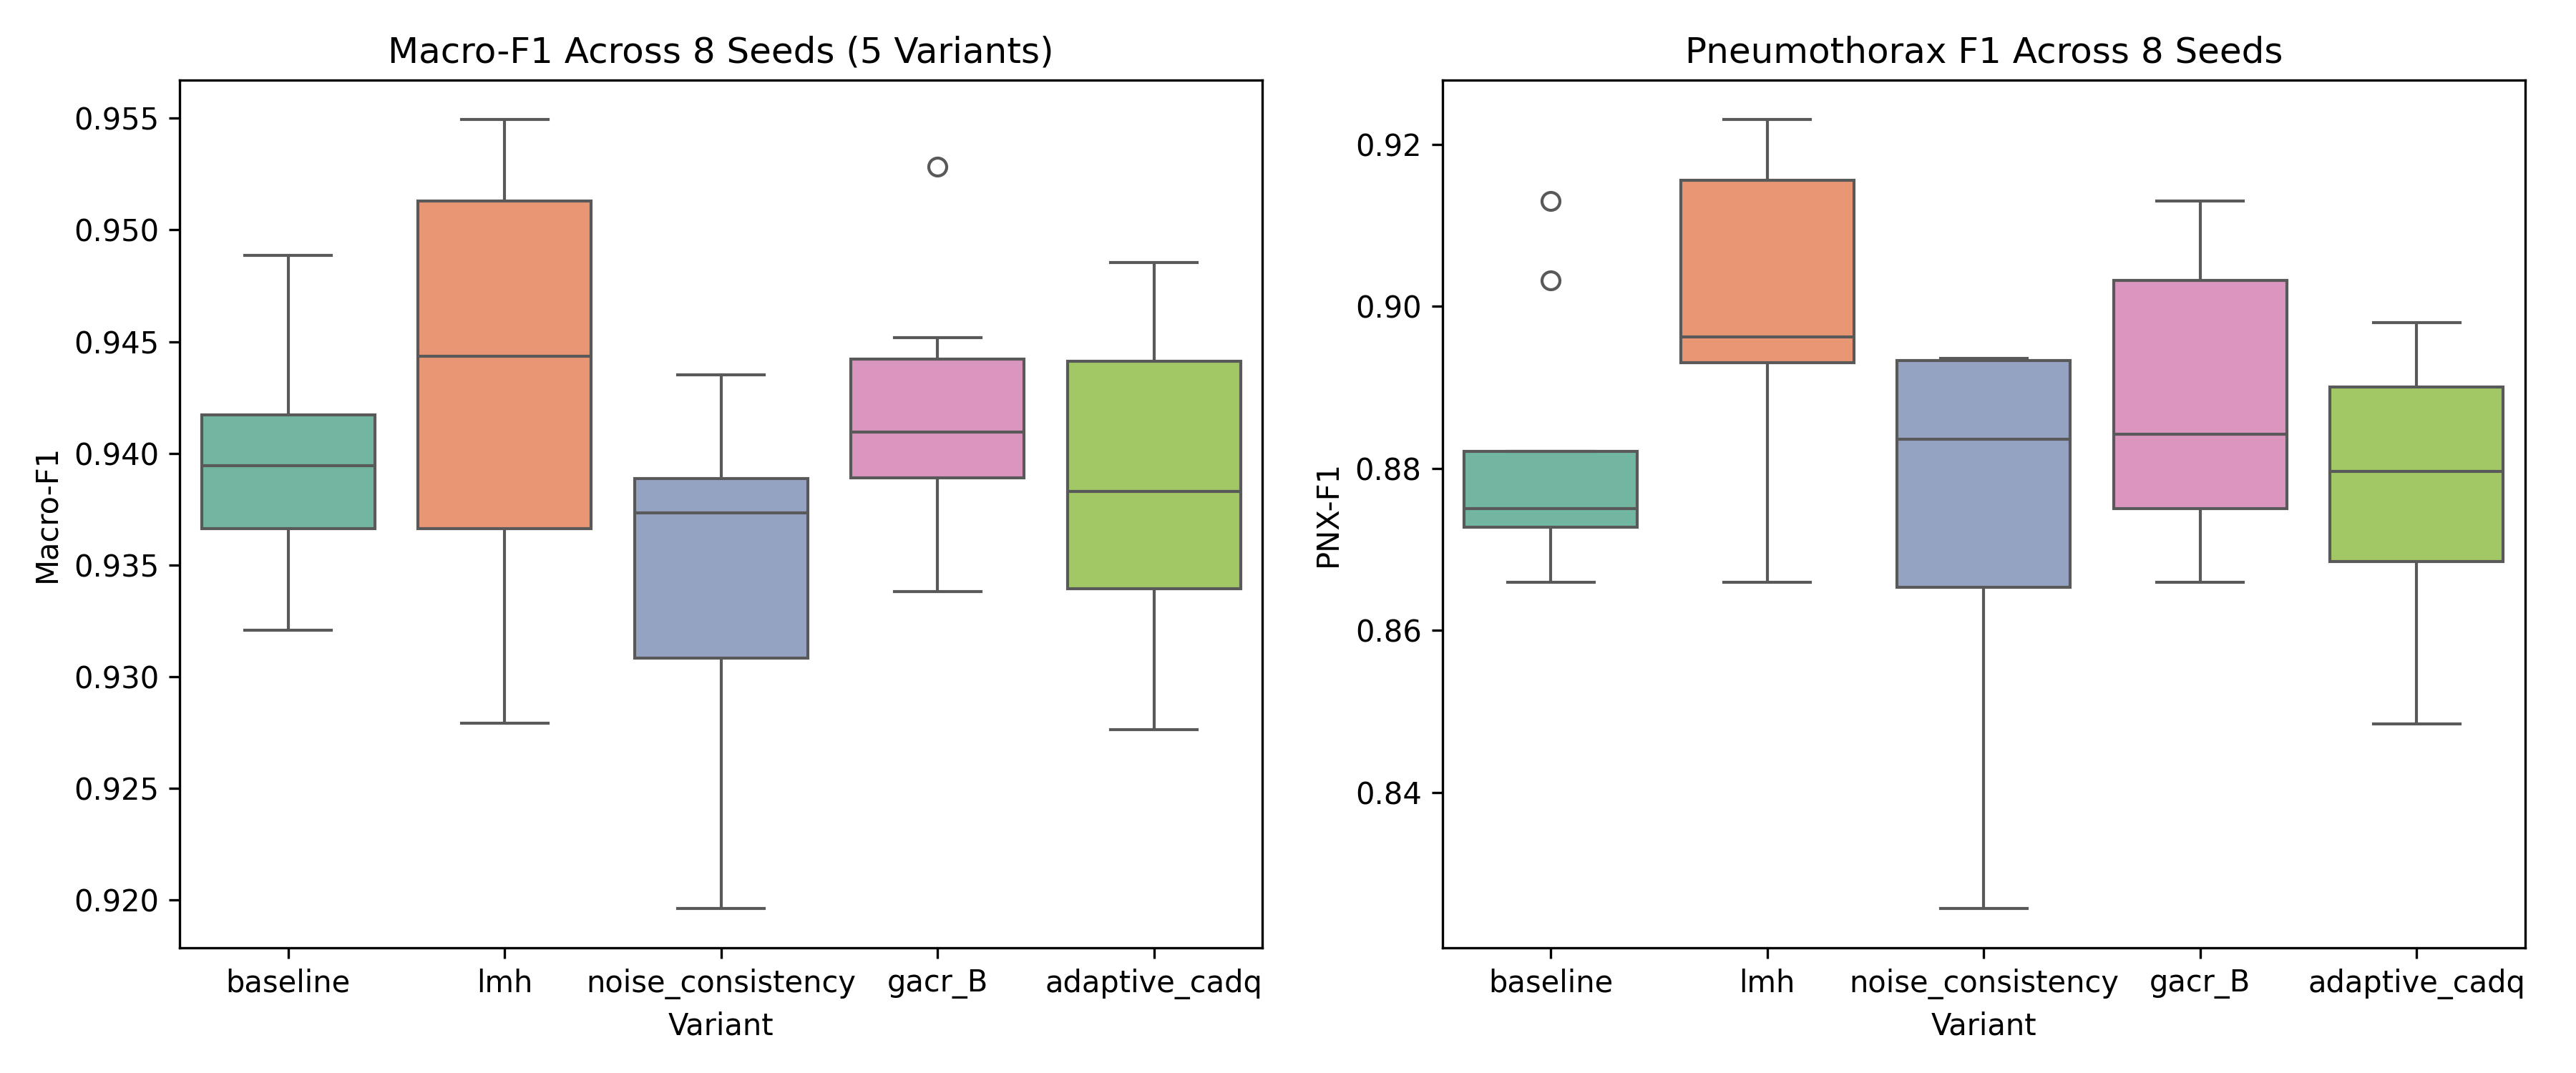
\includegraphics[width=\linewidth]{figures/f1_boxplots.png}
\caption{Macro-F1 and Pneumothorax F1 distributions across eight seeds.}
\label{fig:f1-boxplots}
\end{figure}

No Macro-F1 variant contrast remained significant after Benjamini--Hochberg
correction. The largest unadjusted signal was exploratory GACR-B
($\Delta=+0.0020$, Wilcoxon $p=0.0547$, false-discovery rate (FDR)
$p=0.2188$). LMH reduced AUROC by 0.0126 (FDR $p=0.000012$), and
Noise-Consistency by 0.0014 (FDR $p=0.0044$); Adaptive-CADQ did not differ
from baseline (FDR $p=0.8438$). LMH increased
ECE by 0.0384 and Brier by 0.0163 (FDR $p=0.0313$ and $0.0156$). Noise-
Consistency increased Brier by 0.0133 (FDR $p=0.0156$), while its ECE change
was inconclusive.

\begin{table}[pos=htbp]
\centering
\caption{Paired comparison $p$-values versus Baseline. Wilcoxon tests use
eight seed-level Macro-F1 values; DeLong uses matched Pneumothorax ROC
predictions (seed 42, the retained probability set); McNemar uses paired
classification decisions on the same 455 studies. No predictions were pooled
across seeds. Values in parentheses are Benjamini--Hochberg adjusted within
each test family.}
\label{tab:pairwise-pvalues}
\scriptsize
\resizebox{\linewidth}{!}{%
\begin{tabular}{lccc}
\toprule
Condition & Wilcoxon Macro-F1 $p$ (BH) & DeLong PNX AUROC $p$ (BH) & McNemar $p$ (BH)\\
\midrule
LMH (PoE) & 0.2500 (0.3333) & $<0.0001$ (0.000012) & 0.6936 (1.0000)\\
Noise-Consistency & 0.1953 (0.3333) & 0.0022 (0.0044) & 0.0754 (0.3018)\\
GACR-B (exploratory) & 0.0547 (0.2188) & 0.0315 (0.0420) & 1.0000 (1.0000)\\
Adaptive-CADQ & 0.8438 (0.8438) & 0.7304 (0.7304) & 1.0000 (1.0000)\\
\bottomrule
\end{tabular}}
\end{table}



GACR-B and Adaptive-CADQ produced zero prediction discordance with Baseline
across all 455 held-out studies (McNemar $p=1.000$ for each). Thus, despite
different loss functions and training dynamics, these variants yielded
byte-identical decisions on the test set. This result is consistent with a
text-dominated optimization landscape in which the report shortcut acts as a
single attractor; it is not evidence that the image pathway is intrinsically
non-functional in other cohorts.

Mean row-normalized baseline recalls were 97.78\% (Normal), 95.54\%
(Pneumonia), and 89.36\% (Pneumothorax). LMH improved Normal recall but reduced
Pneumothorax recall; Noise-Consistency showed the reverse trade-off.

\begin{figure}[pos=htbp]
\centering
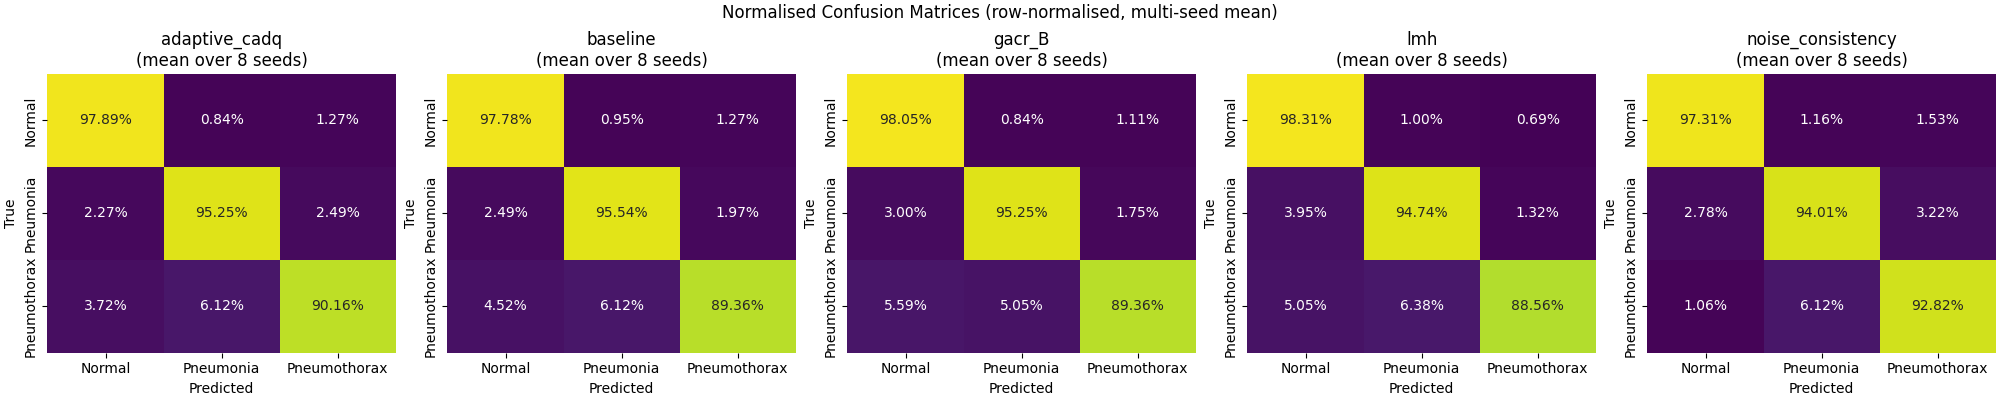
\includegraphics[width=\linewidth]{figures/confusion_matrices_normalised.png}
\caption{Row-normalized confusion matrices aggregated across the eight seeds.
Each matrix is normalized by the true-class row; the displayed aggregate is
descriptive because the same held-out studies recur across seeds.}
\label{fig:confusion-matrices}
\end{figure}

\begin{figure}[pos=htbp]
\centering
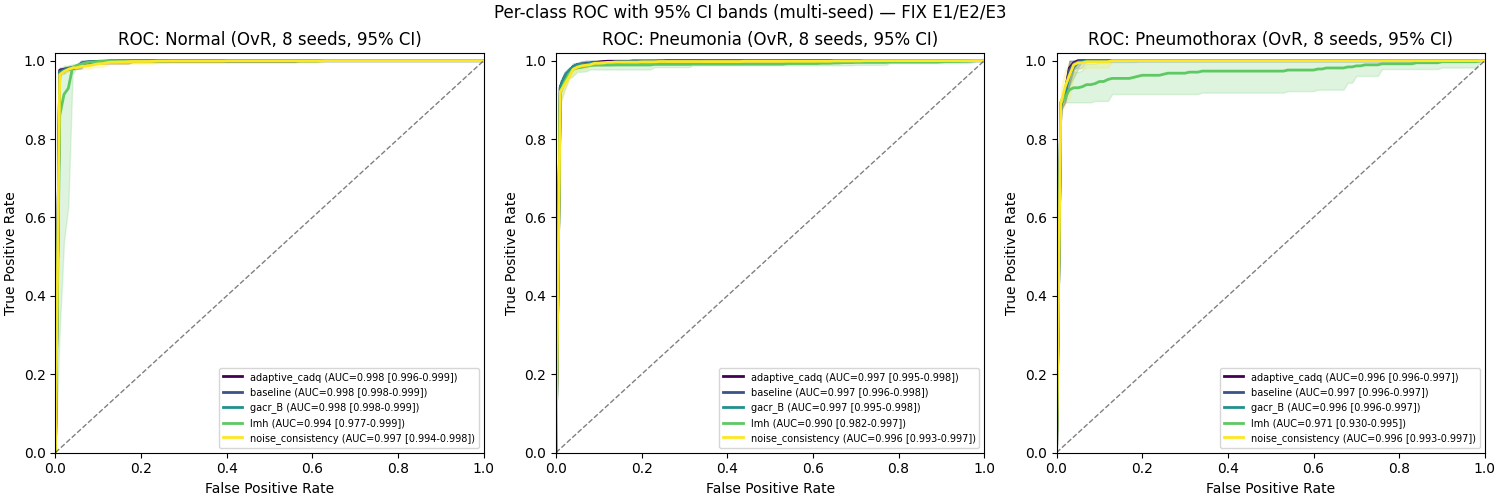
\includegraphics[width=\linewidth]{figures/roc_curves_with_ci.png}
\caption{Per-class ROC curves with descriptive multi-seed 95\% bands. Significant
DeLong $p$-values for LMH and Noise-Consistency reflect AUROC degradation
relative to Baseline, not improvement; all DeLong comparisons use matched
seed-level predictions.}
\label{fig:roc-curves}
\end{figure}

The baseline reliability error was $0.0237\pm0.0048$ and Brier score
$0.0522\pm0.0040$; LMH was less calibrated. Reliability and ROC displays are
descriptive because the same studies recur across seeds.

\begin{figure}[pos=htbp]
\centering
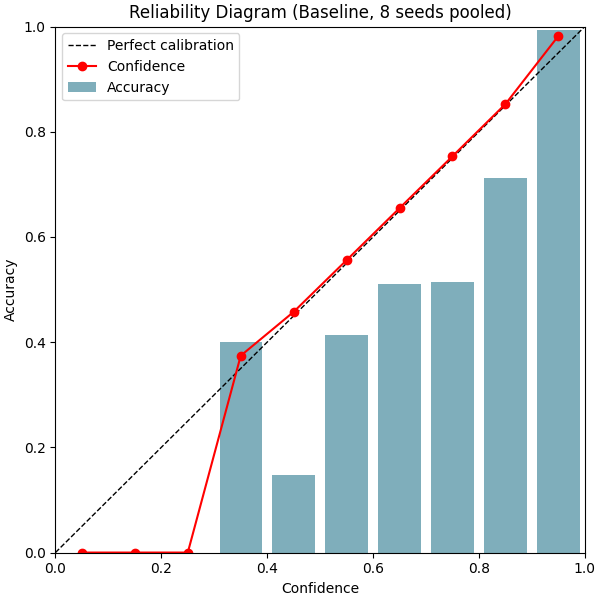
\includegraphics[width=0.50\linewidth]{figures/reliability_diagram.png}
\caption{Descriptive baseline reliability diagram.}
\label{fig:reliability}
\end{figure}

\begin{figure}[pos=htbp]
\centering
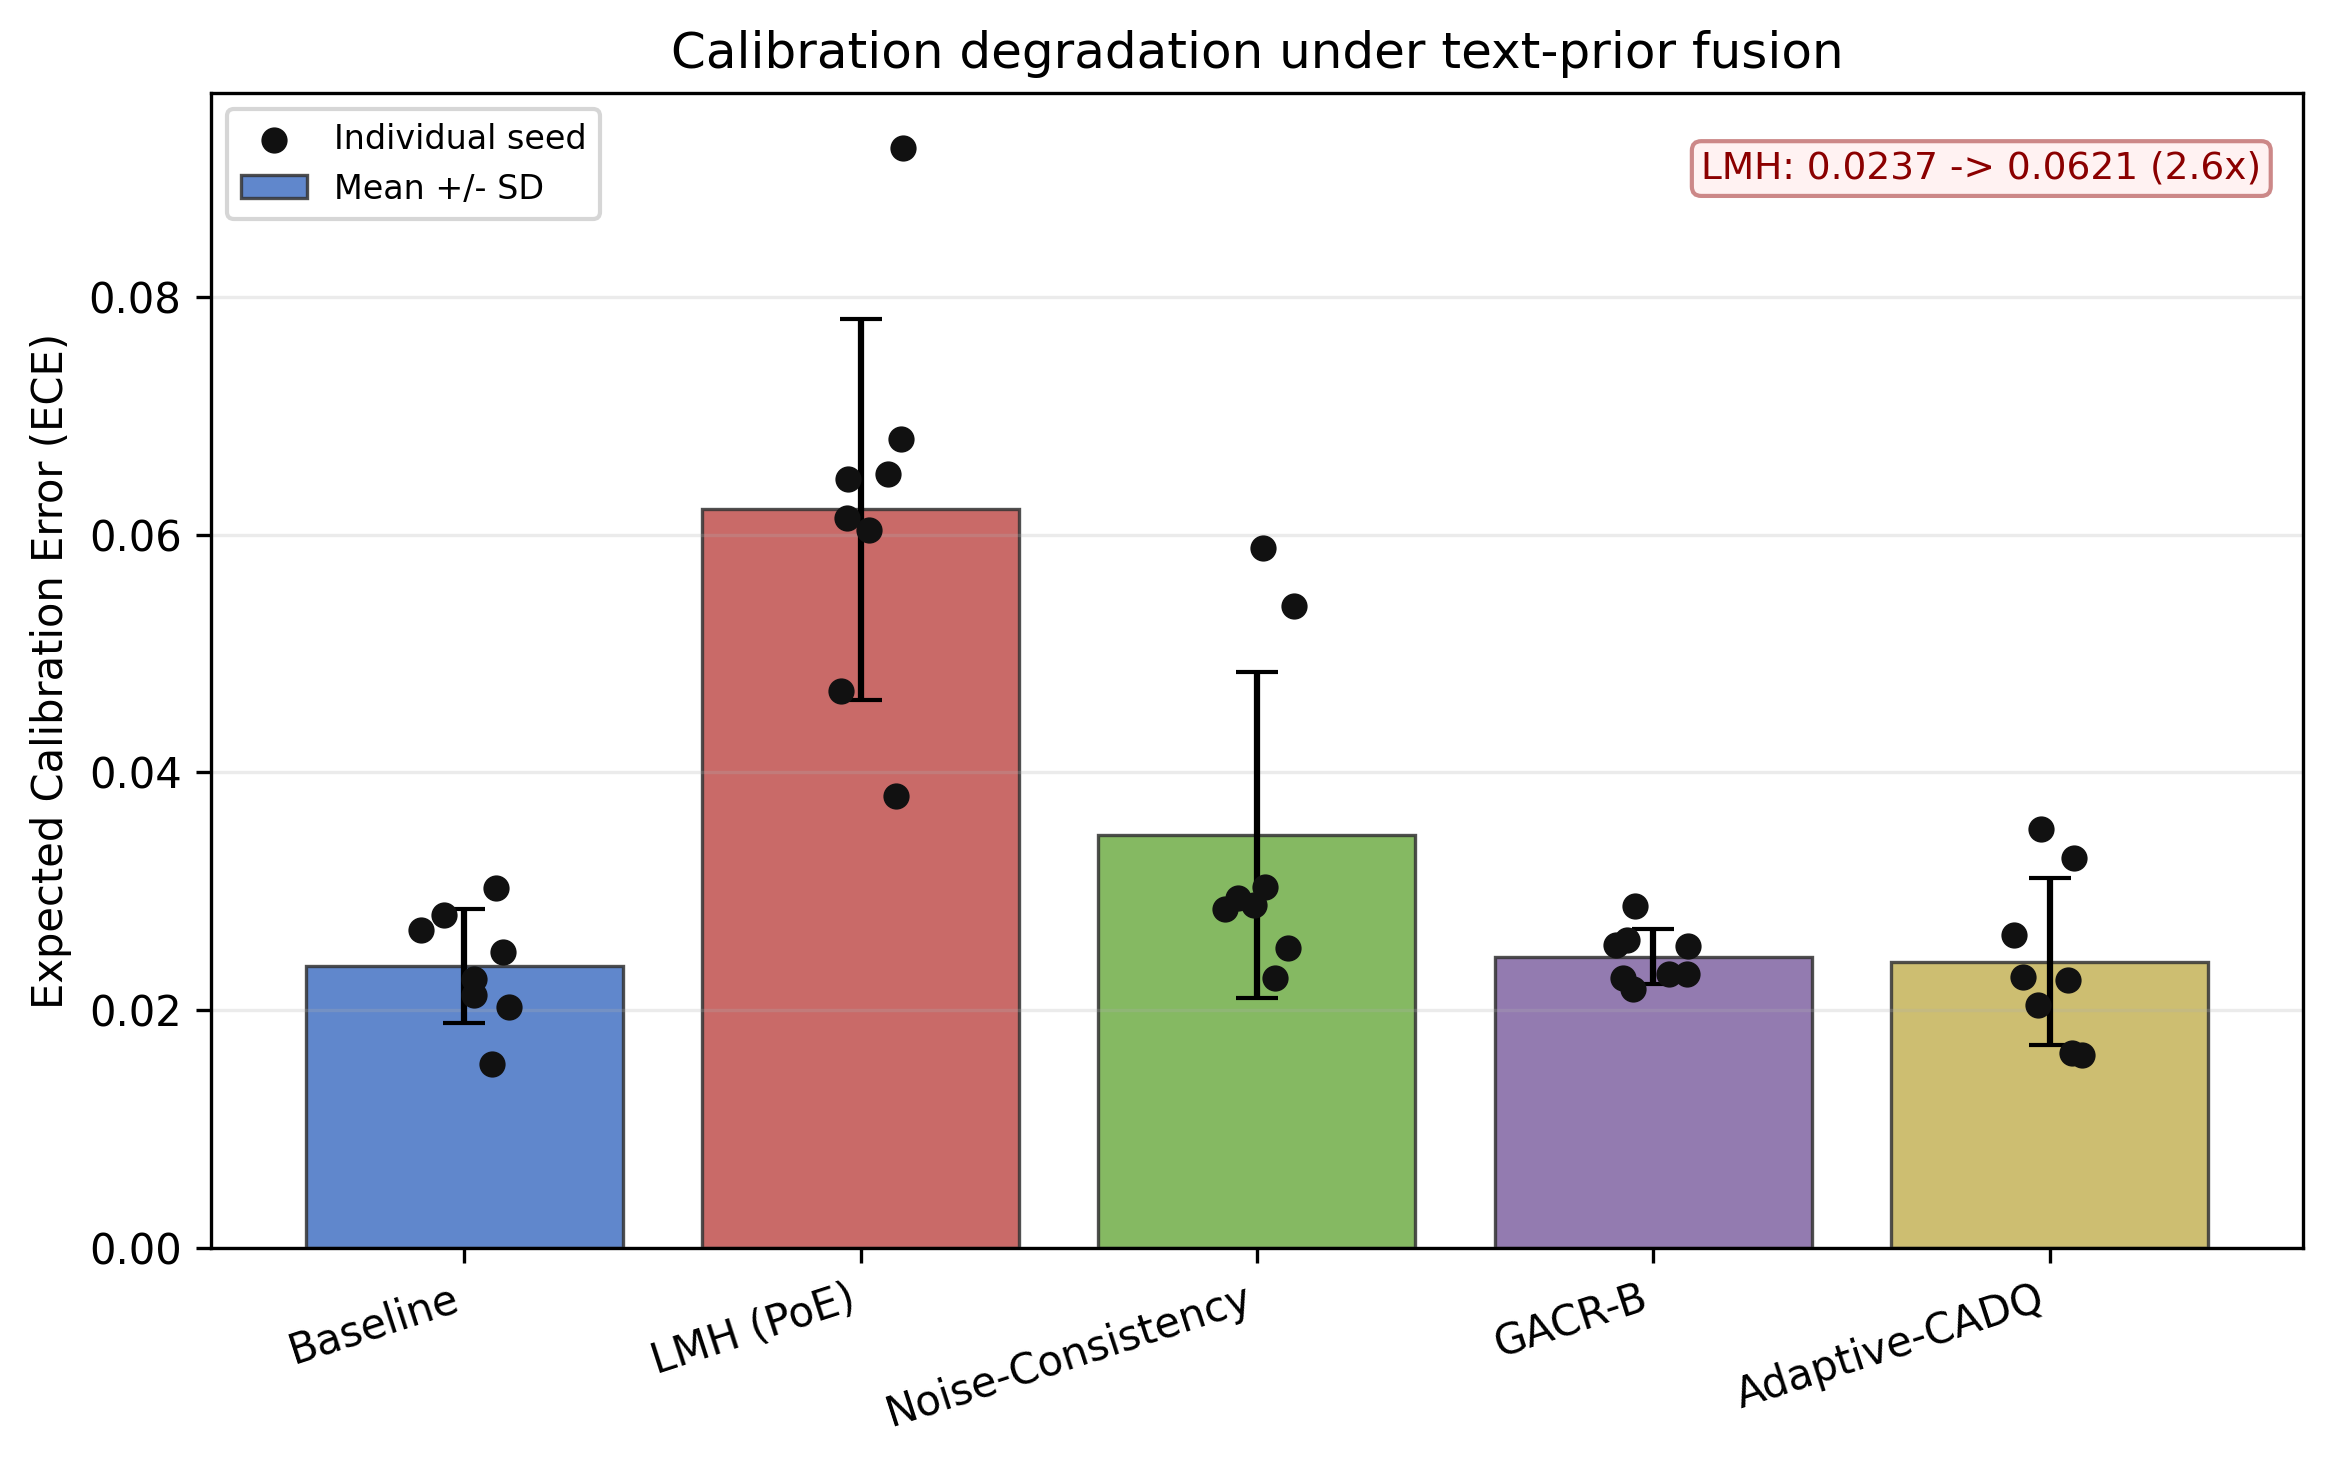
\includegraphics[width=0.68\linewidth]{figures/ece_seed_dots.png}
\caption{Expected calibration error (ECE) by condition with individual seed
values. LMH increases ECE from 0.0237 to 0.0621 (2.6-fold); bars show mean
$\pm$ SD across eight seeds.}
\label{fig:ece-seed-dots}
\end{figure}

\subsection{Controls and report-preserving ablation}\label{sec:results-controls}
The retained image-only control achieved Macro-F1 0.4611, accuracy 0.5670, and
AUROC 0.6728; text-only achieved 0.8555 and 0.9820, respectively. Gray-Square
retained Macro-F1 0.9381, accuracy 0.9604, and AUROC 0.9960, only 0.0015 below
the baseline mean. These are single saved runs, and image-only checkpoint
selection was imperfect, so the controls are diagnostic rather than modality
rankings.

\begin{table}[pos=htbp]
\centering
\caption{Retained control outputs on the 455-study test set (single runs).}
\label{tab:controls}
\small
\begin{tabular}{lccccc}
\toprule
Control & Macro-F1 & Accuracy & Macro-AUROC & ECE & Brier\\
\midrule
Image-only & 0.4611 & 0.5670 & 0.6728 & 0.0993 & 0.6142\\
Text-only & 0.8555 & 0.9077 & 0.9820 & 0.0203 & 0.1289\\
Gray-Square & 0.9381 & 0.9604 & 0.9960 & 0.0369 & 0.0589\\
\bottomrule
\end{tabular}
\end{table}

\begin{figure}[pos=htbp]
\centering
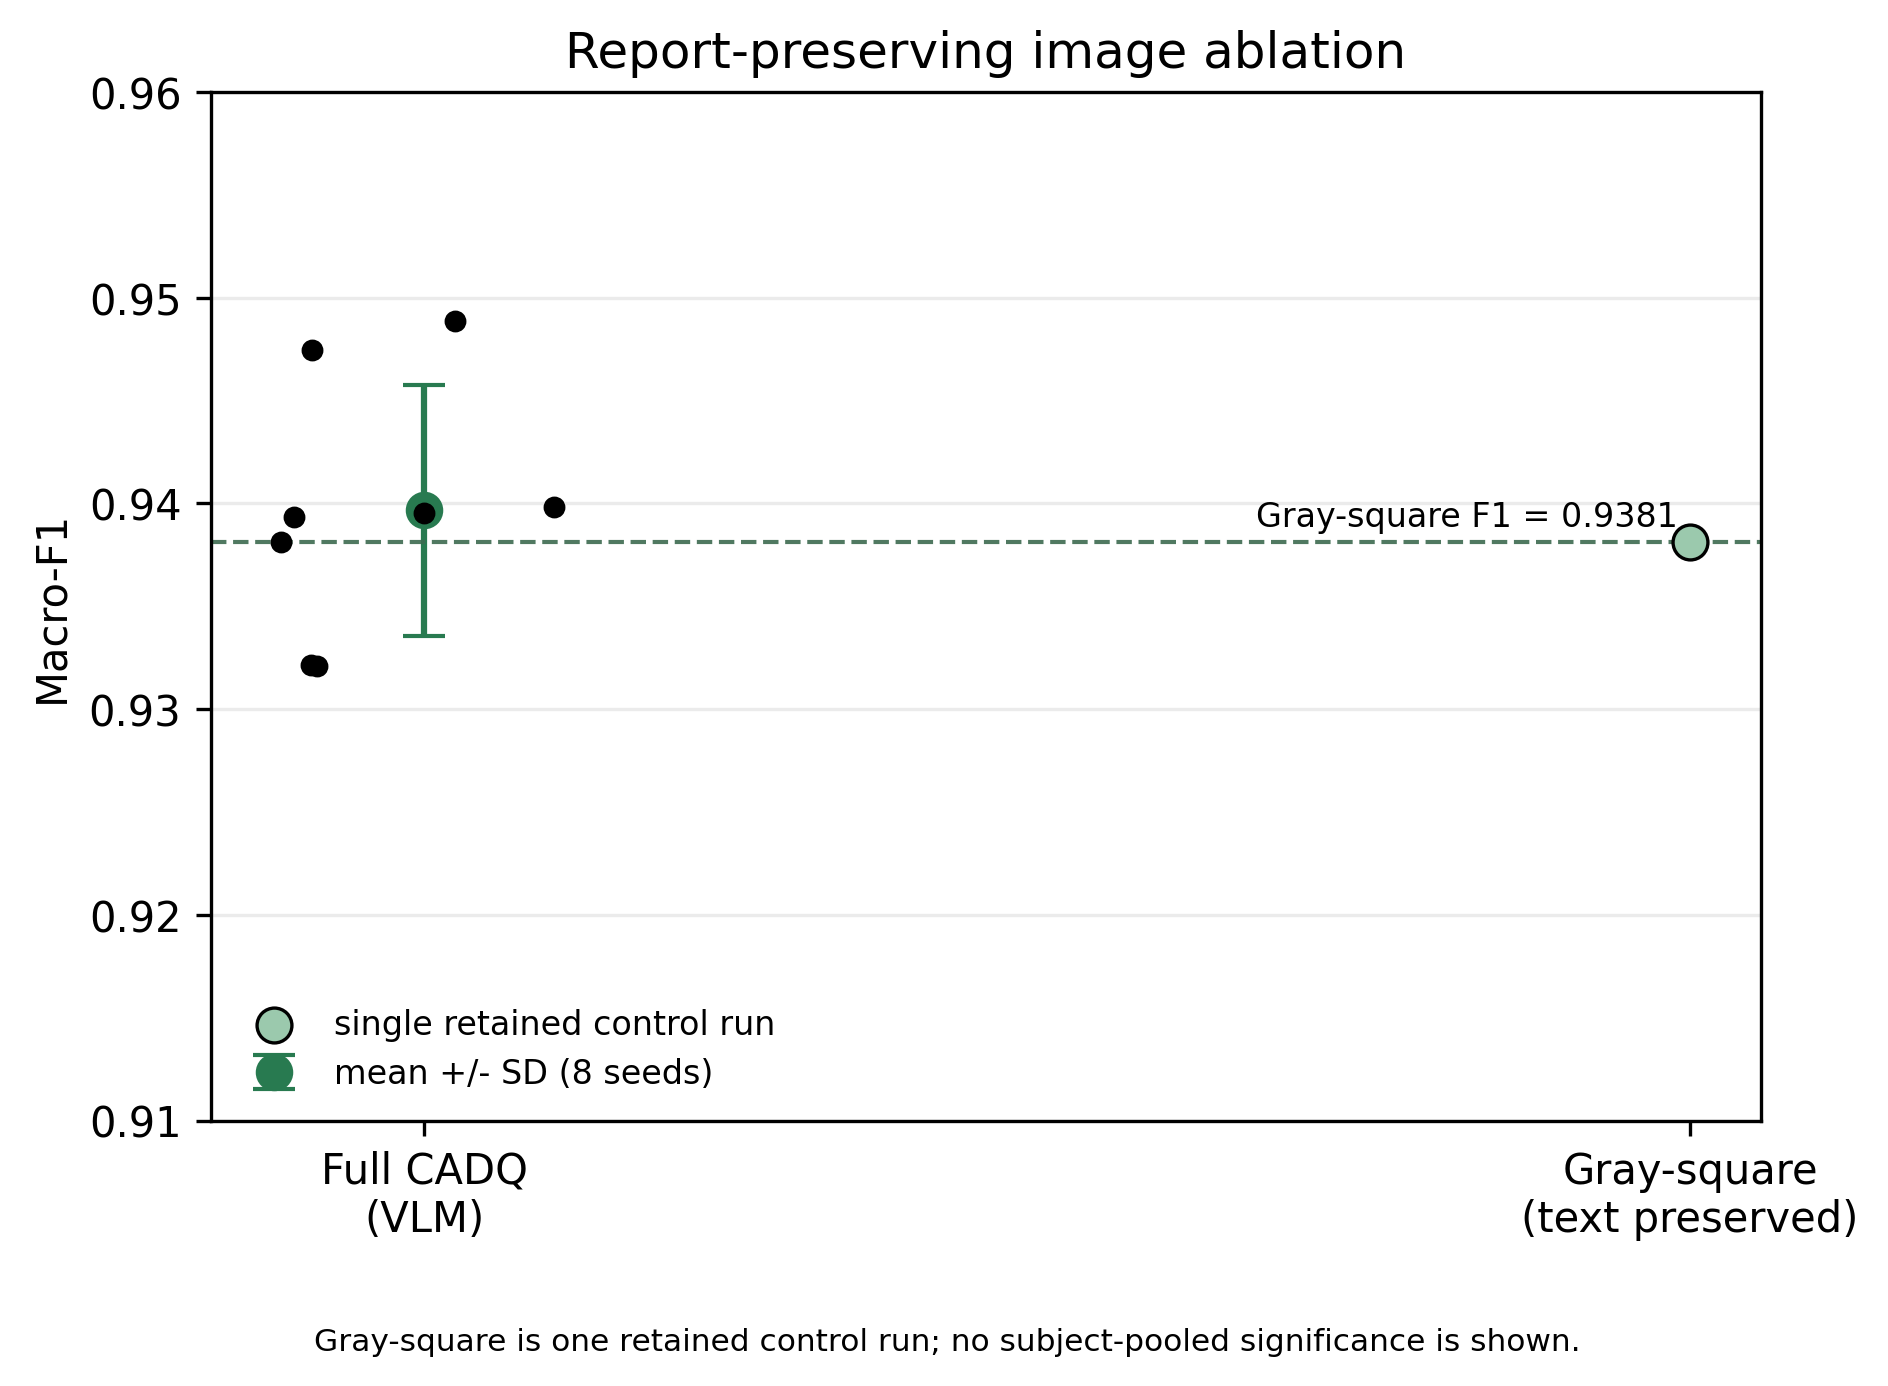
\includegraphics[width=0.66\linewidth]{figures/circularity_contrast.png}
\caption{Report-preserving image ablation; Gray-Square is one retained run.}
\label{fig:circularity-contrast}
\end{figure}

\begin{figure}[pos=htbp]
\centering
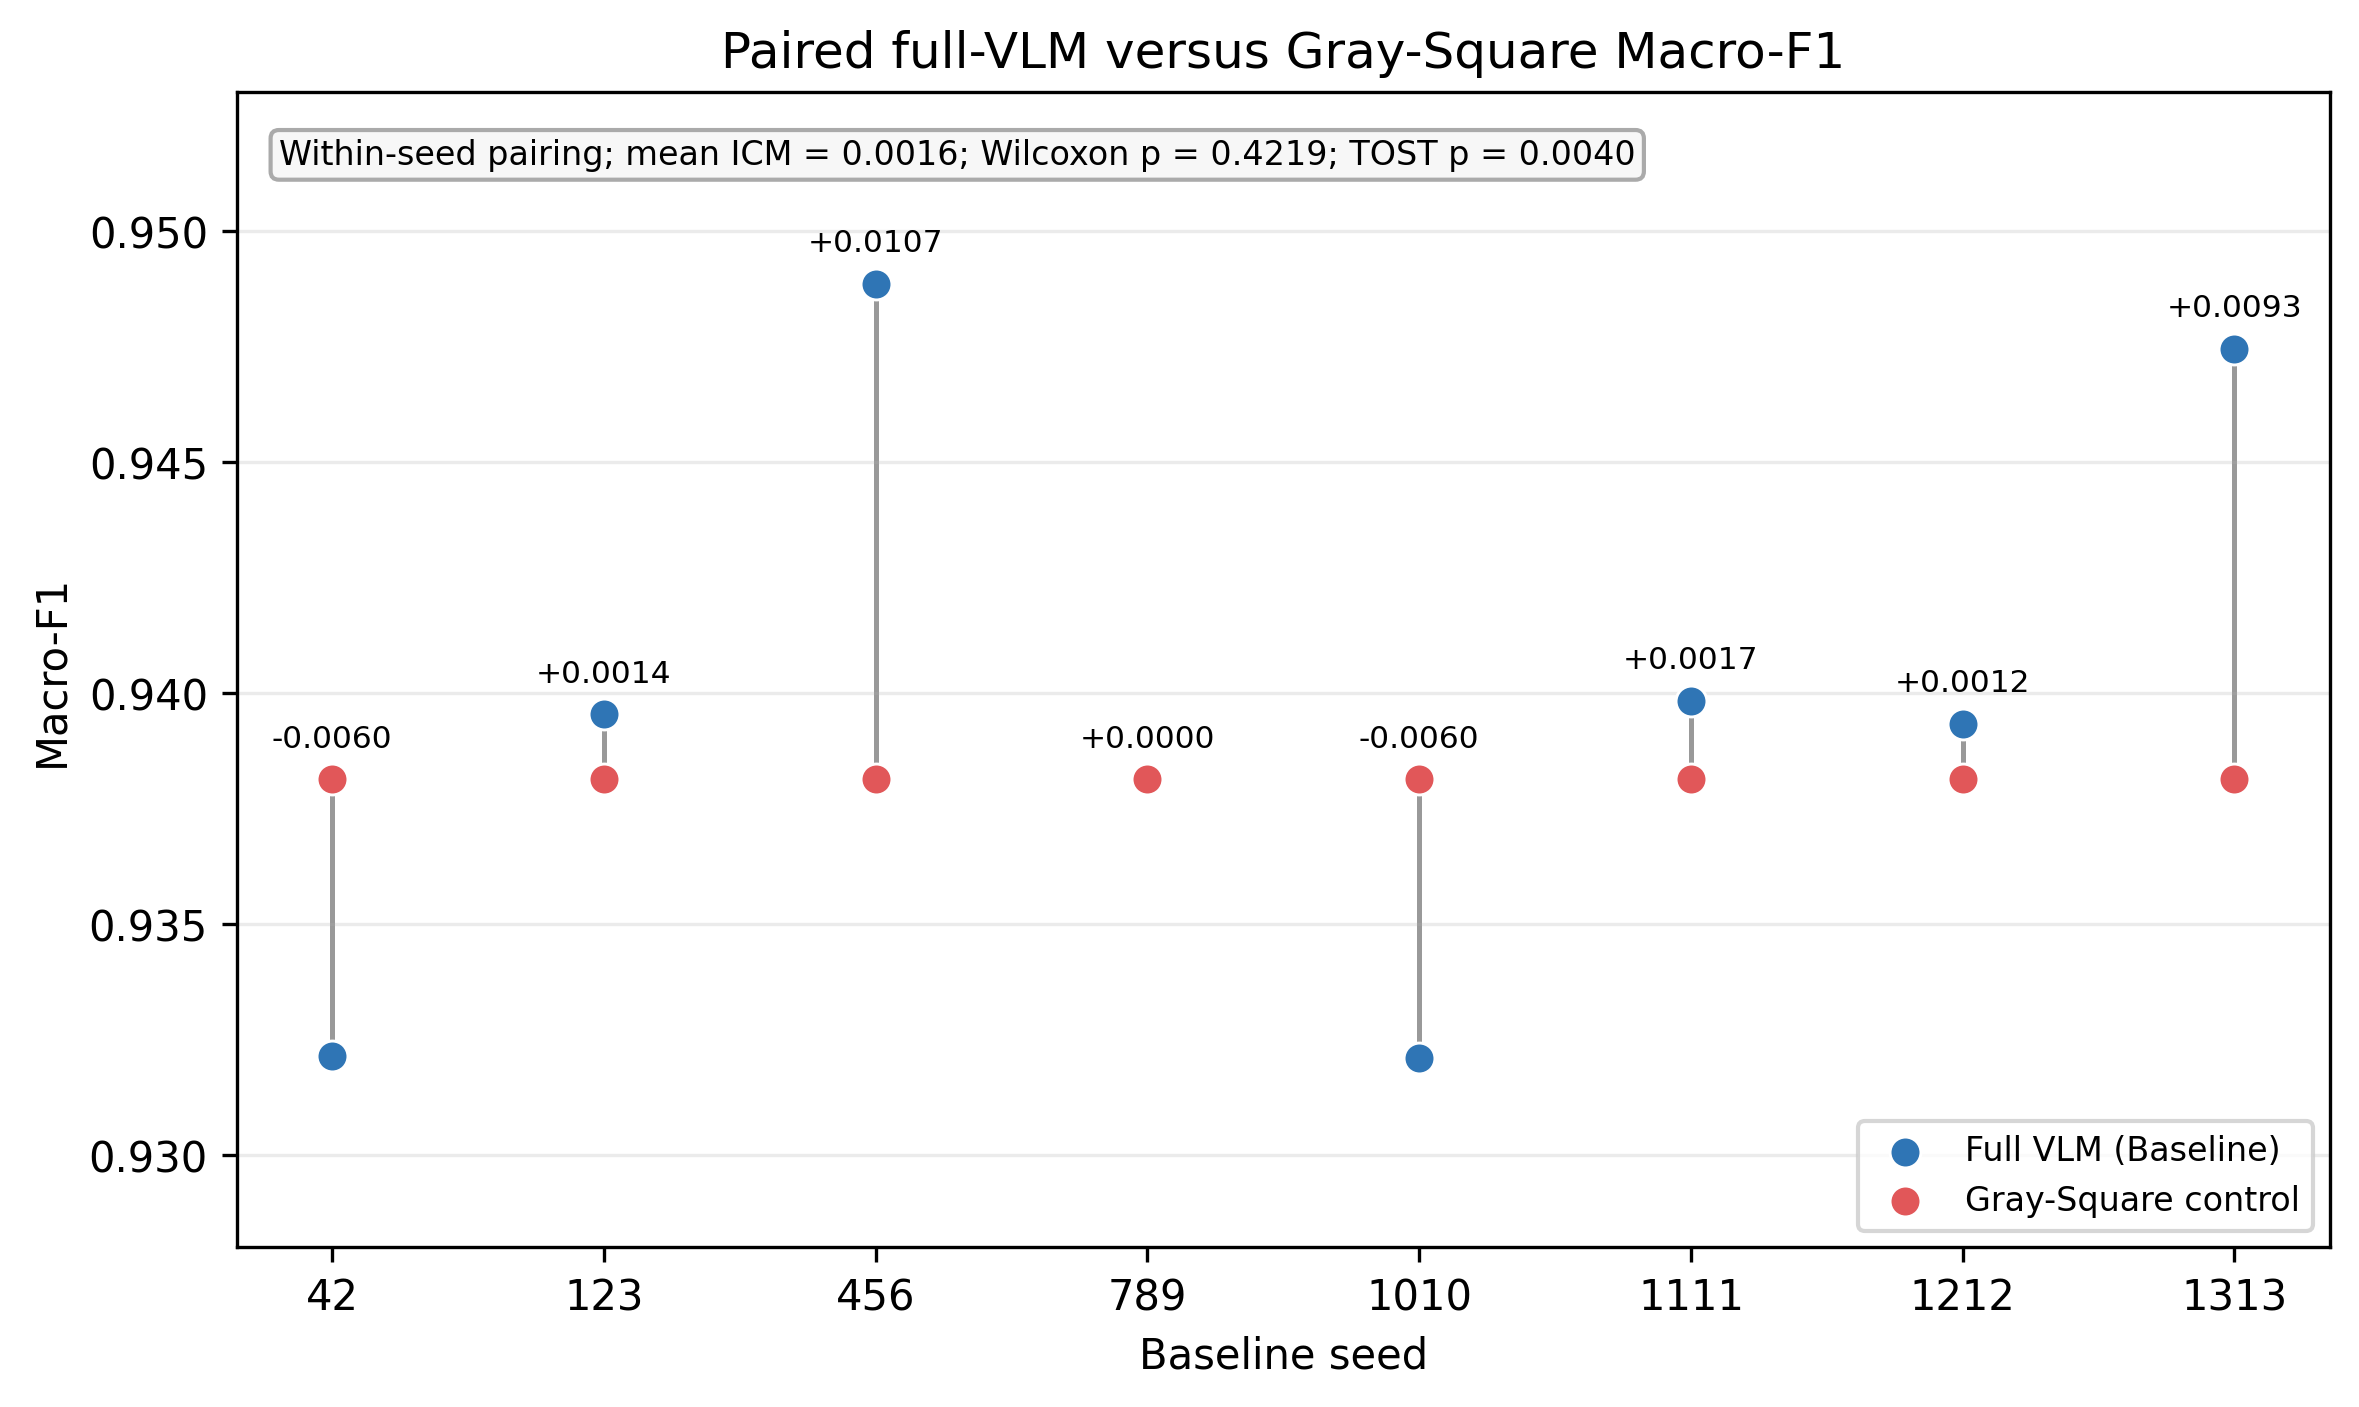
\includegraphics[width=0.70\linewidth]{figures/paired_vlm_gray_square.png}
\caption{Paired Baseline VLM and Gray-Square Macro-F1 for the eight baseline
seeds. Lines connect the two predictions for the same seed; the small paired
differences make the near-zero ICM visible.}
\label{fig:paired-vlm-gray}
\end{figure}

\subsection{Image Contribution Metric}\label{sec:results-icm}
With Gray-Square as reference, baseline ICM was $0.0016\pm0.0065$ (median
0.0014). The bootstrap 95\% confidence interval (CI) was
$[-0.0026,0.0061]$. The signed Wilcoxon test did not
reject zero ($p=0.4219$), while TOST supported equivalence within
$[-0.01,0.01]$ ($p=0.0040$, Cohen’s $d=0.247$). LMH had ICM
$0.0056\pm0.0098$ (TOST $p=0.1223$); Noise-Consistency $-0.0039\pm0.0081$
(TOST $p=0.0345$); Adaptive-CADQ $0.0007\pm0.0077$ (TOST $p=0.0054$); and
exploratory GACR-B $0.0038\pm0.0062$ (TOST $p=0.0122$). None demonstrated a
robust increase in incremental image contribution.

\begin{table}[pos=htbp]
\centering
\caption{Image Contribution Metric (ICM) statistics by condition (eight seeds).
Confidence intervals are percentile bootstrap intervals from 2,000 resamples;
Wilcoxon tests are signed-rank tests against zero; TOST tests equivalence to
zero within $[-0.01,0.01]$.}
\label{tab:icm-statistics}
\scriptsize
\resizebox{\linewidth}{!}{%
\begin{tabular}{lrrrrrrr}
\toprule
Condition & Mean & SD & Median & 95\% CI & Wilcoxon $p$ & TOST $p$ & Cohen's $d$\\
\midrule
Baseline & 0.0016 & 0.0065 & 0.0014 & [-0.0026, 0.0061] & 0.4219 & 0.0040 & 0.247\\
LMH (PoE) & 0.0056 & 0.0098 & 0.0066 & [-0.0011, 0.0118] & 0.1953 & 0.1223 & 0.566\\
Noise-Consistency & -0.0039 & 0.0081 & -0.0009 & [-0.0097, 0.0009] & 0.3828 & 0.0345 & -0.476\\
GACR-B (exploratory) & 0.0038 & 0.0062 & 0.0030 & [-0.0002, 0.0081] & 0.1953 & 0.0122 & 0.607\\
Adaptive-CADQ & 0.0007 & 0.0077 & 0.0002 & [-0.0043, 0.0057] & 0.8438 & 0.0054 & 0.089\\
\bottomrule
\end{tabular}}
\end{table}

\begin{figure}[pos=htbp]
\centering
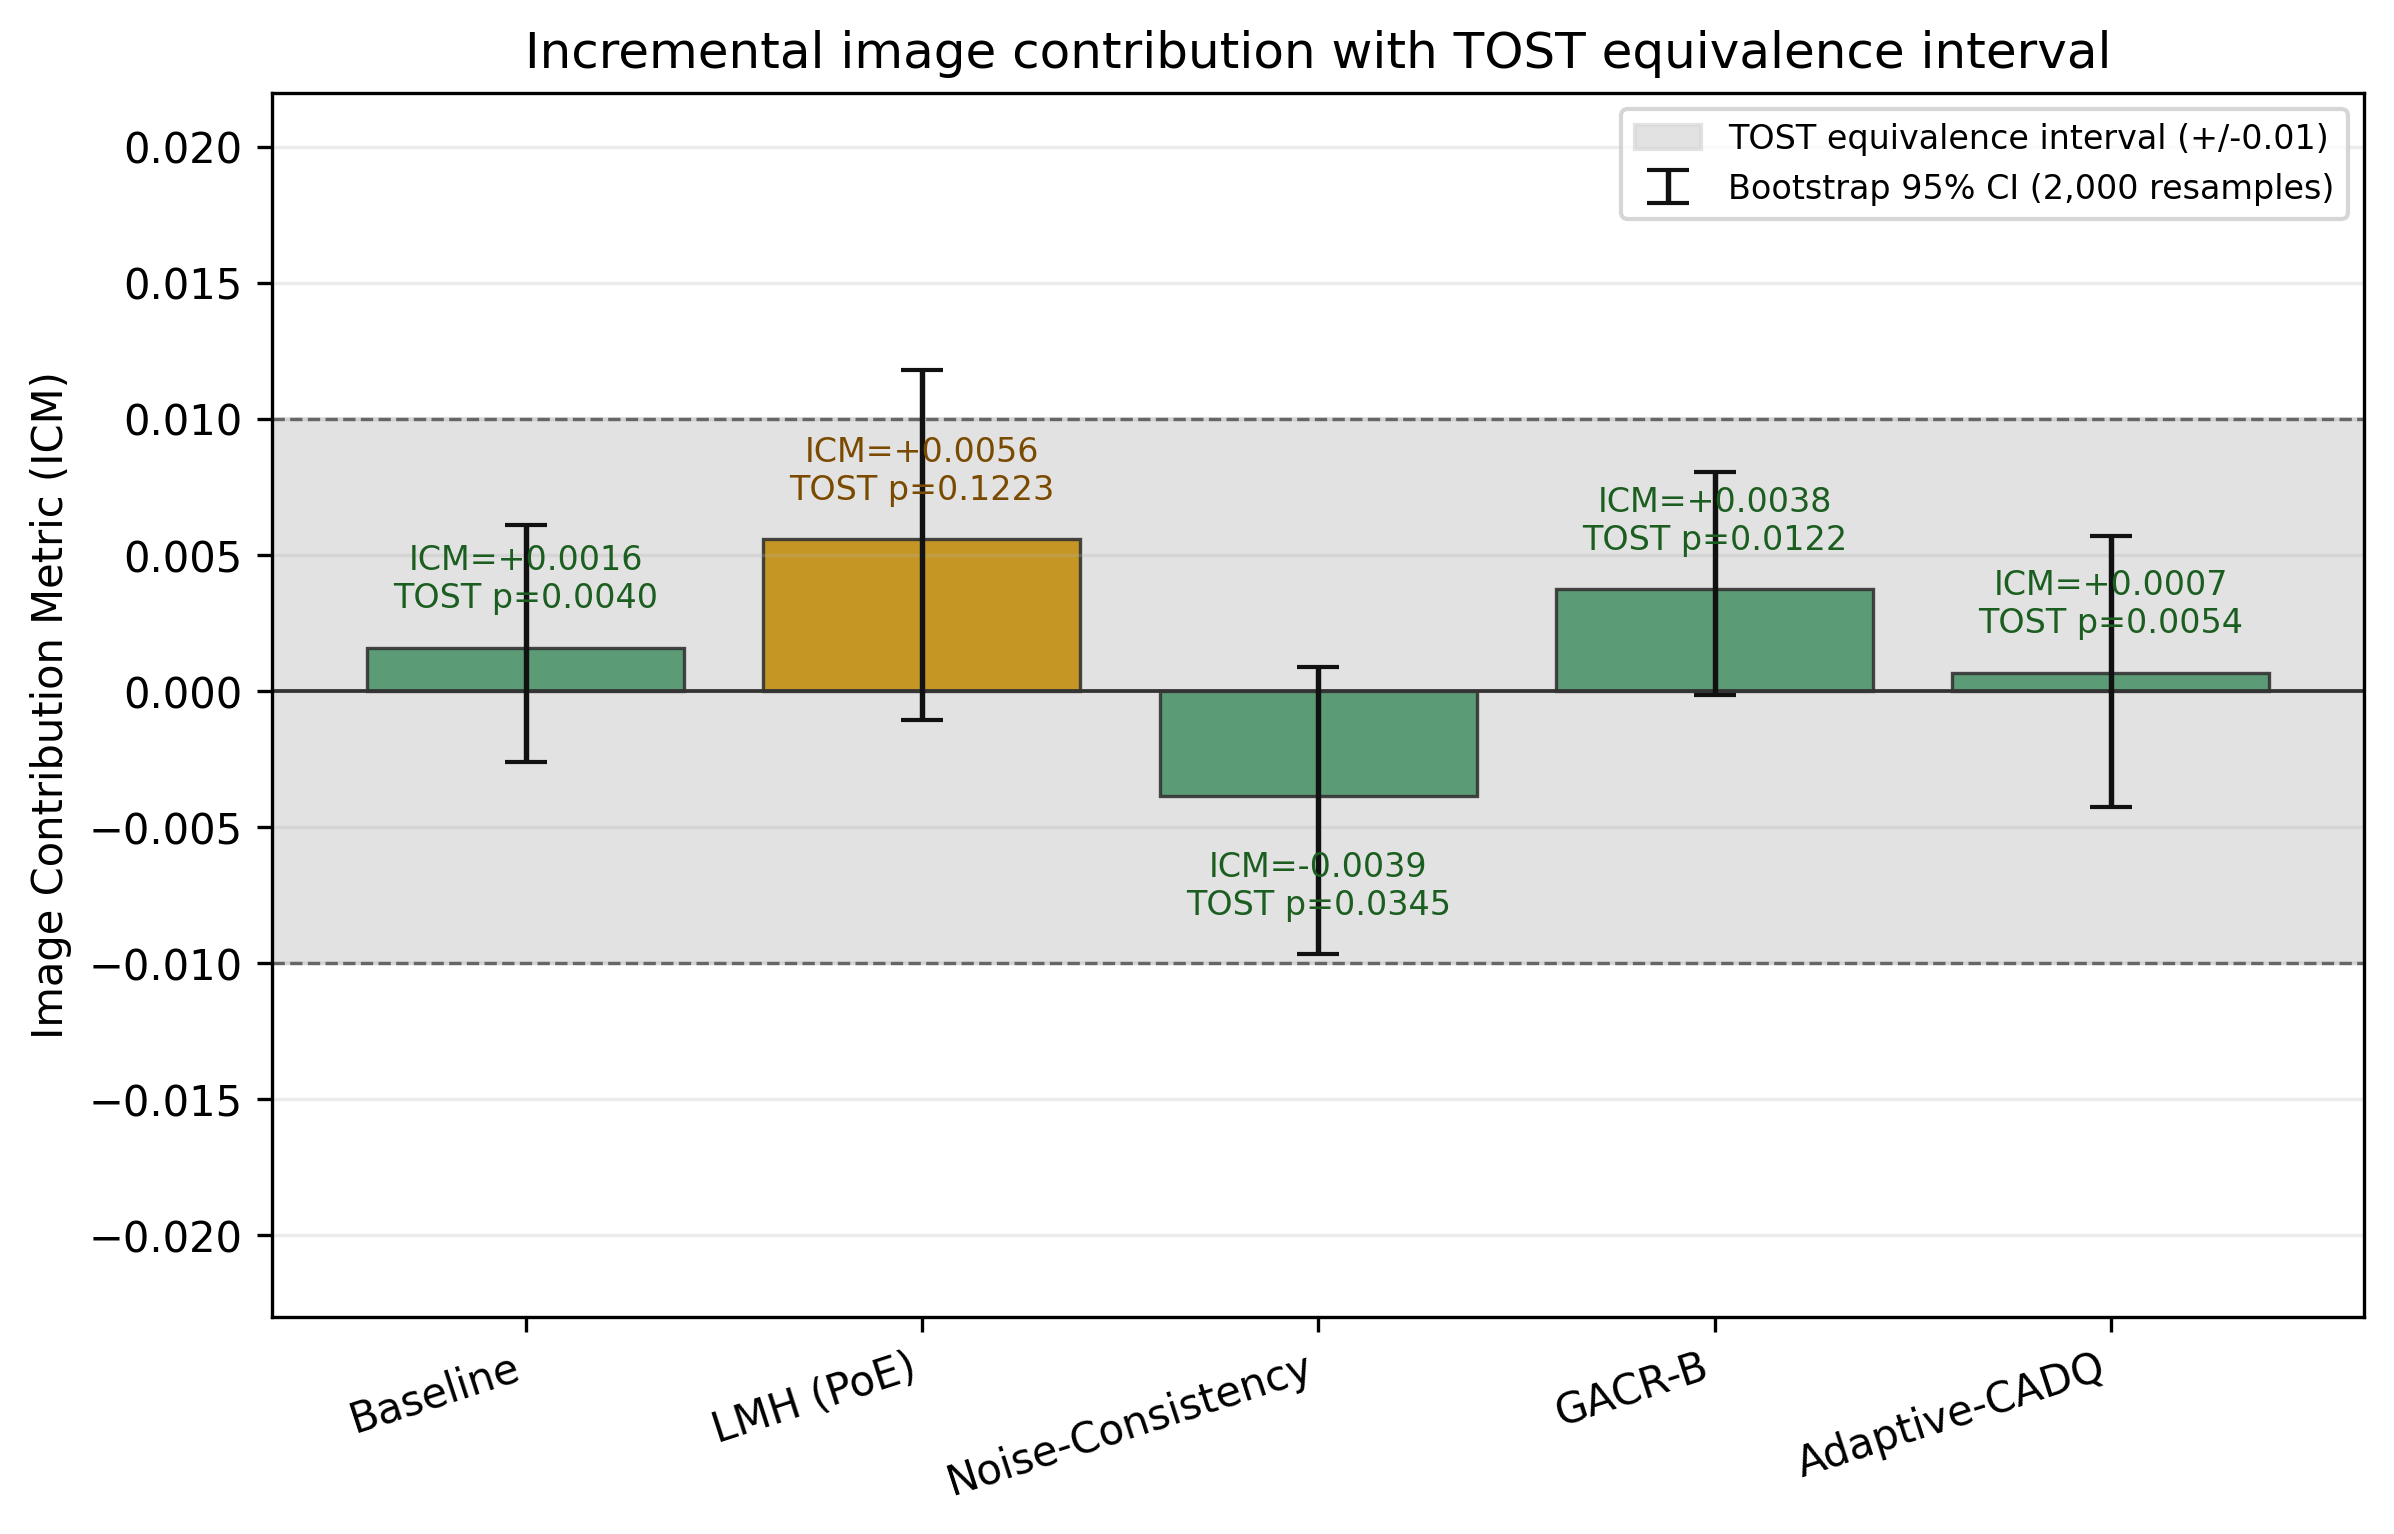
\includegraphics[width=0.70\linewidth]{figures/icm_tost_master.png}
\caption{ICM by condition with percentile bootstrap 95\% confidence intervals.
The shaded band is the pre-specified TOST equivalence interval
$[-0.01,0.01]$; corrected Master statistics are annotated for each condition.}
\label{fig:icm-tost}
\end{figure}

\begin{figure}[pos=htbp]
\centering
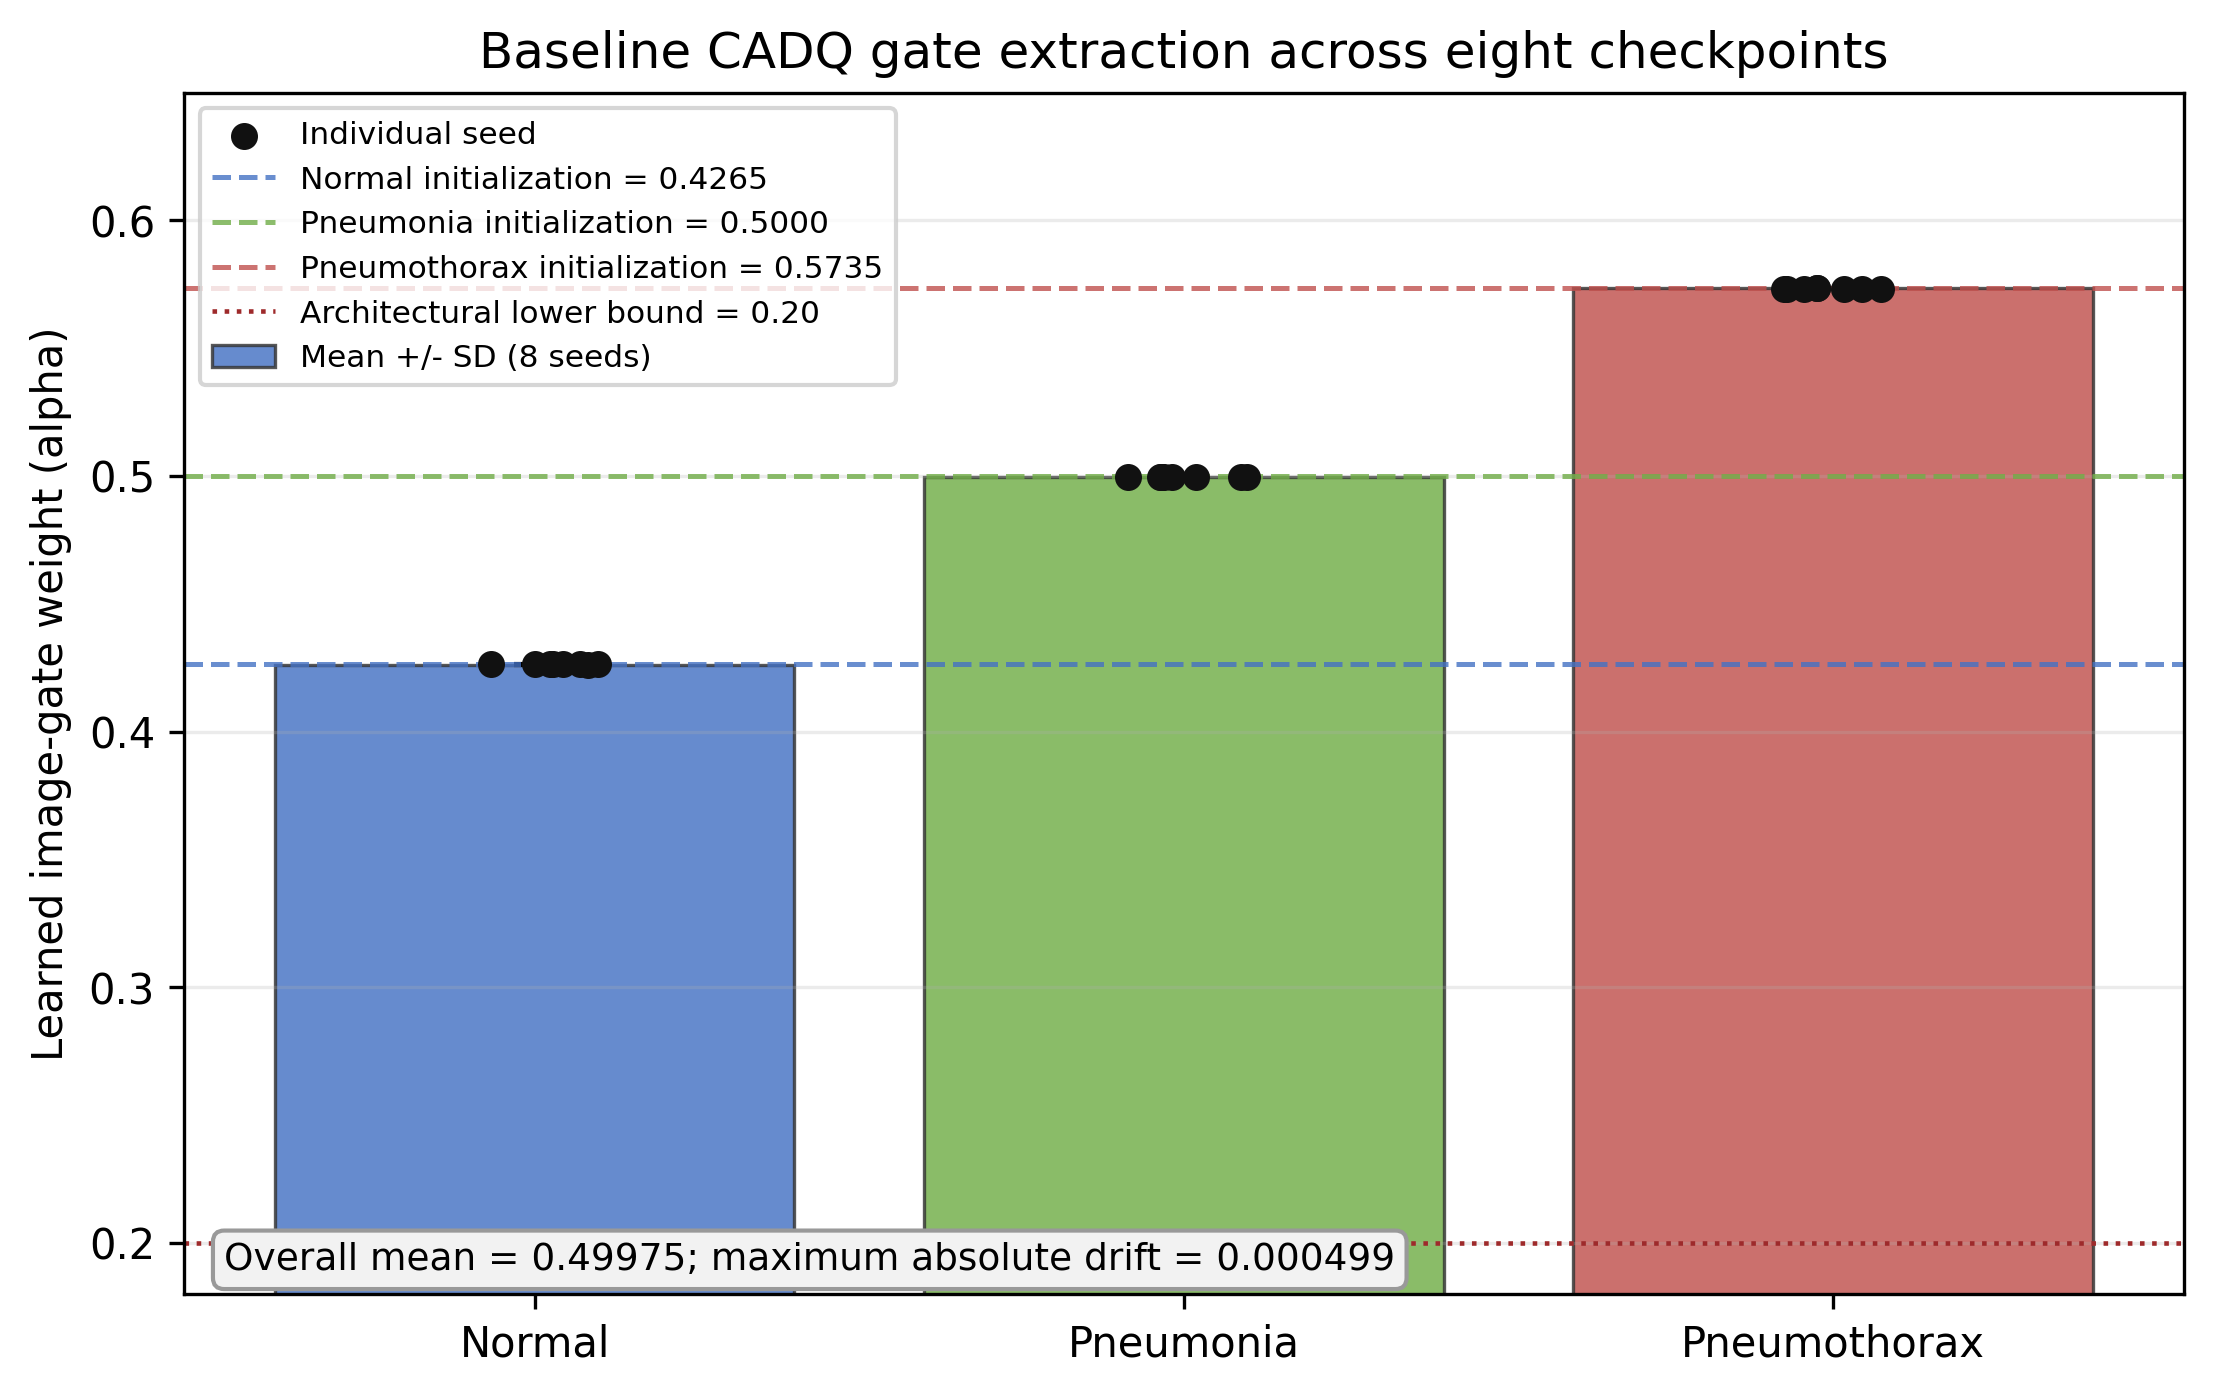
\includegraphics[width=0.70\linewidth]{figures/gate_stagnation_with_dots.png}
\caption{Baseline CADQ image-gate weights extracted from eight checkpoints.
Bars show mean $\pm$ SD, dots show individual seeds, and dashed lines show the
class-specific initialization values computed from the saved checkpoint logits.}
\label{fig:gate-stagnation}
\end{figure}

\subsection{Fusion gates and qualitative inspection}\label{sec:results-gate}
Extracted baseline image-gate means were 0.42624 (Normal), 0.49963
(Pneumonia), and 0.57336 (Pneumothorax), with overall mean 0.49975 versus
0.50000 at initialization. The largest class-wise drift was below 0.0004; the
gate neither collapsed to 0.20 nor demonstrated learned image reliance. Three
Pneumonia Grad-CAM examples (Fig.~\ref{fig:gradcam}) are qualitative only and
do not support localization or causal-grounding claims.

\begin{table}[pos=htbp]
\centering
\caption{Per-seed CADQ gate extraction. Initialization values are computed from
$u=(-0.5,0,0.5)$ and the bounded gate equation; maximum drift is the largest
absolute class-wise deviation from initialization for that seed.}
\label{tab:gate-extraction}
\scriptsize
\setlength{\tabcolsep}{4pt}
\begin{tabular}{r rrr r}
\toprule
Seed & Normal $\alpha$ & Pneumonia $\alpha$ & Pneumothorax $\alpha$ & Max drift\\
\midrule
42   & 0.426270 & 0.499512 & 0.573242 & 0.000488\\
123  & 0.426270 & 0.499512 & 0.573730 & 0.000488\\
456  & 0.426025 & 0.499756 & 0.573242 & 0.000499\\
789  & 0.426270 & 0.499756 & 0.573242 & 0.000255\\
1010 & 0.426270 & 0.499756 & 0.573242 & 0.000255\\
1111 & 0.426270 & 0.499512 & 0.573242 & 0.000488\\
1212 & 0.426270 & 0.499756 & 0.573730 & 0.000255\\
1313 & 0.426270 & 0.499512 & 0.573242 & 0.000488\\
\bottomrule
\end{tabular}
\end{table}

\begin{figure}[pos=htbp]
\centering

\includegraphics[width=0.74\linewidth]{figures/gradcam_baseline.png}
\caption{Qualitative Grad-CAM examples (method of Selvaraju et al. \citep{selvaraju2017gradcam}); no quantitative localization claim.}
\label{fig:gradcam}
\end{figure}

Overall, high performance persisted after image replacement, baseline ICM was
near zero, and the gate remained near initialization. This pattern is
consistent with report-linked shortcut potential in this cohort, not a
universal claim that multimodal models ignore images.
